\documentclass[../../main.tex]{subfiles}
\graphicspath{{../../image/}{../../figure/}}
\begin{document}

\section{同族波相互作用}\label{section:ch15-同族波相互作用}

本节给出\eqref{align:ch15-15421}右端第二、三项的估计，它们由同族黏性波的相互作用所诱导。目标是证明：当\eqref{align:ch15-1527}与\eqref{align:ch15-15420}对 $t\in[\bar t,T)$ 成立时，
\begin{align}
\int_{\bar t}^{T}\int_{-\infty}^{\infty}|\omega_i\partial_xw_i-w_i\partial_x\omega_i|\,dx\,dt=O(\delta_0^2),
\label{align:ch15-1561}
\end{align}
\begin{align}
\int_{\bar t}^{T}\int_{-\infty}^{\infty}\left|w_i\partial_x\left(\frac{\omega_i}{w_i}\right)\right|^2\chi_{\{|\lambda_i^*+\omega_i/w_i|<3\delta_1\}}\,dx\,dt=O(\delta_0^3).
\label{align:ch15-1562}
\end{align}
此目标通过监控解的两个泛函的时间演化而达到，它们具有非常有趣的几何解释。

考虑方程组
\begin{align}
\begin{cases}
\partial_tw(x,t)+\partial_x\left[\sigma(x,t)w(x,t)\right]-\partial_x^2w(x,t)=\varphi(x,t),\\
\partial_t\omega(x,t)+\partial_x\left[\sigma(x,t)\omega(x,t)\right]-\partial_x^2\omega(x,t)=\psi(x,t),
\end{cases}
\label{align:ch15-1563}
\end{align}
在 $[\bar t,T)$ 上的解 $(w,\omega)$，其中 $\varphi$、$\psi$ 与 $\sigma$ 为给定光滑函数，$\varphi(\cdot,t)$ 与 $\psi(\cdot,t)\in L^1(-\infty,\infty)$。于是 $w(\cdot,t)$ 与 $\omega(\cdot,t)$ 也属于 $L^1(-\infty,\infty)$，从而可定义泛函
\begin{align}
\mathscr{L}(t)=\int_{-\infty}^{\infty}\left[w^2(x,t)+\omega^2(x,t)\right]^{1/2}\,dx,
\label{align:ch15-1564}
\end{align}
\begin{align}
\mathscr{A}(t)=\frac12\int_{-\infty}^{\infty}\int_{x<y}|w(x,t)\omega(y,t)-\omega(x,t)w(y,t)|\,dx\,dy.
\label{align:ch15-1565}
\end{align}

引入向量场
\begin{align}
Z(x,t)=\left(\int_{-\infty}^xw(y,t)\,\mathrm{d}y,\ \int_{-\infty}^x\omega(y,t)\,\mathrm{d}y\right).
\label{align:ch15-1566}
\end{align}
对固定的 $t\in[\bar t,T)$，$Z(\cdot,t)$ 定义了 $\mathbb{R}^2$ 上一条以 $x$ 为参数的曲线，因而 $Z$ 表示 $\mathbb{R}^2$ 上一条运动曲线。我们用撇表示沿该曲线关于参数 $x$ 的微分，$'=\partial_x$。注意 $\mathscr{L}(t)$ 是时刻 $t$ 曲线的长度。进而，
\begin{align}
\frac12\int_{-\infty}^{\infty}Z(y,t)\wedge Z'(y,t)\,\mathrm{d}y=\frac12\int_{-\infty}^{\infty}\int_{x<y}Z'(x,t)\wedge Z'(y,t)\,dx\,dy
\label{align:ch15-1567}
\end{align}
给出曲线 $Z(\cdot,t)$ 所围区域面积之和，每块乘以相应的绕数。因而 $\mathscr{A}(t)$ 给出 $Z(\cdot,t)$ 凸包面积的一个上界。

由\eqref{align:ch15-1563}，
\begin{align}
\partial_tZ(x,t)+\sigma(x,t)\partial_xZ(x,t)-\partial_x^2Z(x,t)=\Phi(x,t),
\label{align:ch15-1568}
\end{align}
其中
\begin{align}
\Phi(x,t)=\left(\int_{-\infty}^x\varphi(y,t)\,\mathrm{d}y,\ \int_{-\infty}^x\psi(y,t)\,\mathrm{d}y\right).
\label{align:ch15-1569}
\end{align}
我们的计划是证明：$\mathscr{L}(t)$ 与 $\mathscr{A}(t)$ 的增长率由 $\|\varphi(\cdot,t)\|_{L^1(-\infty,\infty)}$ 与 $\|\psi(\cdot,t)\|_{L^1(-\infty,\infty)}$ 控制；特别地，当 $\varphi$ 与 $\psi$ 恒为零时，这两个泛函非增。

\begin{lemma}\label{lemma:ch15-面积泛函估计}
\begin{align}
\frac{\mathrm{d}}{\mathrm{d}t}\mathscr{A}(t)&\leqslant-\int_{-\infty}^{\infty}|\omega(x,t)\partial_xw(x,t)-w(x,t)\partial_x\omega(x,t)|\,dx\nonumber\\
&\quad+\|w(\cdot,t)\|_{L^1(-\infty,\infty)}\|\psi(\cdot,t)\|_{L^1(-\infty,\infty)}+\|\omega(\cdot,t)\|_{L^1(-\infty,\infty)}\|\varphi(\cdot,t)\|_{L^1(-\infty,\infty)}.
\label{align:ch15-15610}
\end{align}
\end{lemma}

\begin{figure}[ht]
\centering
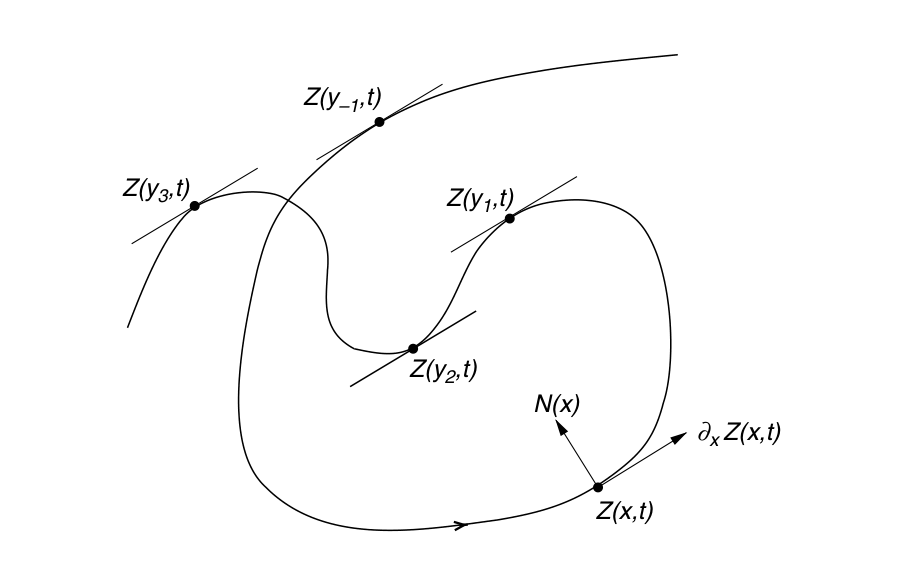
\includegraphics[width=0.85\textwidth]{ch15-fig06-01.png}
\caption{曲线 $Z(\cdot,t)$ 及其在临界点处的法向量 $N(x)$}\label{figure:ch15-曲线与法向量}
\end{figure}

\begin{proof}
固定 $t\in[\bar t,T)$，考虑 $\mathbb{R}^2$ 中曲线 $Z(\cdot,t)$（见\cref{figure:ch15-曲线与法向量}）。对任一 $x\in(-\infty,\infty)$，赋予 $\mathbb{R}^2$ 中单位向量 $N(x)$，它垂直于切向量 $Z'(x,t)$，并由
\begin{align}
Z'(x,t)\wedge N(x)=|Z'(x,t)|
\label{align:ch15-15611}
\end{align}
定向。特别地，对任意 $W\in\mathbb{R}^2$，
\begin{align}
Z'(x,t)\wedge W=|Z'(x,t)|\,[N(x)\cdot W].
\label{align:ch15-15612}
\end{align}

现计算
\begin{align}
\frac{\mathrm{d}}{\mathrm{d}t}\mathscr{A}(t)&=\frac12\int_{-\infty}^{\infty}\int_{x<y}\operatorname{sgn}[Z'(x,t)\wedge Z'(y,t)]\left[\partial_tZ'(x,t)\wedge Z'(y,t)+Z'(x,t)\wedge\partial_tZ'(y,t)\right]dx\,dy\nonumber\\
&=\frac12\int_{-\infty}^{\infty}\int_{-\infty}^{\infty}\operatorname{sgn}[Z'(x,t)\wedge Z'(y,t)]\,[Z'(x,t)\wedge\partial_tZ'(y,t)]\,dy\,dx\nonumber\\
&=\frac12\int_{-\infty}^{\infty}\int_{-\infty}^{\infty}|Z'(x,t)|\operatorname{sgn}\partial_yz(y,x,t)\,\partial_t\partial_yz(y,x,t)\,dy\,dx\nonumber\\
&=\frac12\int_{-\infty}^{\infty}|Z'(x,t)|\,\partial_tTV_{(-\infty,\infty)}z(\cdot,x,t)\,dx,
\label{align:ch15-15613}
\end{align}
其中我们采用记号
\begin{align}
z(y,x,t)=N(x)\cdot Z(y,t).
\label{align:ch15-15614}
\end{align}
由于 $N(x)\cdot Z'(x,t)=0$，$x$ 是 $z(\cdot,x,t)$ 的临界点。为简单起见，设有有限多个临界点 $y_{-p}<\cdots<y_{-1}<y_0=x<y_1<\cdots<y_q$，且无一退化。由于极小与极大交替，
\begin{align}
\operatorname{sgn}\partial_y^2z(y_r,x,t)=(-1)^r\operatorname{sgn}\partial_y^2z(x,x,t).
\label{align:ch15-15615}
\end{align}
简单计算给出
\begin{align}
\partial_tTV_{(-\infty,\infty)}z(\cdot,x,t)=-2\sum_{-p\leqslant r\leqslant q}\operatorname{sgn}\partial_y^2z(y_r,x,t)\,\partial_tz(y_r,x,t).
\label{align:ch15-15616}
\end{align}
将 $\partial_tz=N\cdot\partial_tZ$ 代入\eqref{align:ch15-15616}，其中 $\partial_tZ$ 取自\eqref{align:ch15-1568}。由于 $\partial_yz(y_r,x,t)=0$，并由\eqref{align:ch15-15615}，
\begin{align}
\partial_tTV_{(-\infty,\infty)}z(\cdot,x,t)=-2\sum_{-p\leqslant r\leqslant q}|\partial_y^2z(y_r,x,t)|-2\operatorname{sgn}\partial_y^2z(x,x,t)\sum_{-p\leqslant r\leqslant q}(-1)^r[N(x)\cdot\Phi(y_r,t)].
\label{align:ch15-15617}
\end{align}
进而，
\begin{align}
\sum_{-p\leqslant r\leqslant q}|\partial_y^2z(y_r,x,t)|\geqslant|\partial_y^2z(y_0,x,t)|=|N(x)\cdot Z''(x,t)|,
\label{align:ch15-15618}
\end{align}
\begin{align}
\left|\sum_{-p\leqslant r\leqslant q}(-1)^r[N(x)\cdot\Phi(y_r,t)]\right|\leqslant\int_{-\infty}^{\infty}|N(x)\cdot\Phi'(y,t)|\,\mathrm{d}y.
\label{align:ch15-15619}
\end{align}

联合\eqref{align:ch15-15613}、\eqref{align:ch15-15617}、\eqref{align:ch15-15618}、\eqref{align:ch15-15619}、\eqref{align:ch15-15614}与\eqref{align:ch15-15612}，得
\begin{align}
\frac{\mathrm{d}}{\mathrm{d}t}\mathscr{A}(t)\leqslant-\int_{-\infty}^{\infty}Z'(x,t)\wedge Z''(x,t)\,\mathrm{d}x+\int_{-\infty}^{\infty}\int_{-\infty}^{\infty}|Z'(x,t)\wedge\Phi'(y,t)|\,\mathrm{d}y\,\mathrm{d}x.
\label{align:ch15-15620}
\end{align}
由于 $Z'=(w,\omega)$ 且 $\Phi'=(\varphi,\psi)$，\eqref{align:ch15-15620}给出\eqref{align:ch15-15610}。证明完成。
\end{proof}

\begin{lemma}\label{lemma:ch15-长度泛函估计}
在假设 $w^2+\omega^2\neq0$ 下，
\begin{align}
\frac{\mathrm{d}}{\mathrm{d}t}\mathscr{L}(t)&\leqslant-\frac1{(1+9\delta_1^2)^{3/2}}\int_{-\infty}^{\infty}|w(x,t)|\,\left|\partial_x\left(\frac{\omega(x,t)}{w(x,t)}\right)\right|^2\chi_{\{|\omega/w|<3\delta_1\}}\,\mathrm{d}x\nonumber\\
&\quad+\|\varphi(\cdot,t)\|_{L^1(-\infty,\infty)}+\|\psi(\cdot,t)\|_{L^1(-\infty,\infty)}.
\label{align:ch15-15621}
\end{align}
\end{lemma}

\begin{proof}
由于 $w^2+\omega^2\neq0$，
\begin{align}
\frac{\mathrm{d}}{\mathrm{d}t}\mathscr{L}(t)=\int_{-\infty}^{\infty}\frac{w\partial_tw+\omega\partial_t\omega}{(w^2+\omega^2)^{1/2}}\,\mathrm{d}x.
\label{align:ch15-15622}
\end{align}
把\eqref{align:ch15-1563}中的 $\partial_tw$ 与 $\partial_t\omega$ 代入\eqref{align:ch15-15622}。利用初等恒等式
\begin{align}
\frac{w\partial_x(\sigma w)+\omega\partial_x(\sigma\omega)}{(w^2+\omega^2)^{1/2}}=\partial_x\left[\sigma(w^2+\omega^2)^{1/2}\right],
\label{align:ch15-15623}
\end{align}
\begin{align}
\frac{w\partial_x^2w+\omega\partial_x^2\omega}{(w^2+\omega^2)^{1/2}}=\partial_x^2(w^2+\omega^2)^{\frac12}-\frac{|w|\,\left|\partial_x\left(\frac{\omega}{w}\right)\right|^2}{\left[1+\left(\frac{\omega}{w}\right)^2\right]^{3/2}},
\label{align:ch15-15624}
\end{align}
得
\begin{align}
\frac{\mathrm{d}}{\mathrm{d}t}\mathscr{L}(t)=-\int_{-\infty}^{\infty}\frac{|w|\,\left|\partial_x\left(\frac{\omega}{w}\right)\right|^2}{\left[1+\left(\frac{\omega}{w}\right)^2\right]^{3/2}}\,\mathrm{d}x+\int_{-\infty}^{\infty}\frac{w\varphi+\omega\psi}{(w^2+\omega^2)^{1/2}}\,\mathrm{d}x,
\label{align:ch15-15625}
\end{align}
由此易见\eqref{align:ch15-15621}。证明完成。
\end{proof}

为证明\eqref{align:ch15-1561}，在 $[\bar t,T)$ 上积分\eqref{align:ch15-15610}得估计
\begin{align}
\int_{\bar t}^{T}\int_{-\infty}^{\infty}|\omega(x,t)\partial_xw(x,t)-w(x,t)\partial_x\omega(x,t)|\,dx\,dt&\leqslant\mathscr{A}(\bar t)\nonumber\\
&\quad+\sup_{[\bar t,T)}\left(\|w(\cdot,t)\|_{L^1(-\infty,\infty)}+\|\omega(\cdot,t)\|_{L^1(-\infty,\infty)}\right)\nonumber\\
&\quad\times\int_{\bar t}^{T}\int_{-\infty}^{\infty}\bigl(|\varphi(x,t)|+|\psi(x,t)|\bigr)\,dx\,dt.
\label{align:ch15-15626}
\end{align}
回顾\eqref{align:ch15-1526}，对 $w=w_i$，$\omega=\omega_i$，$\varphi=\varphi_i$，$\psi=\psi_i$，$\sigma=\sigma_i$ 应用\eqref{align:ch15-15626}。此时，由\eqref{align:ch15-1527}与原书 (15.4.23)，

为验证\eqref{align:ch15-1562}，在 $[\bar t,T)$ 上积分\eqref{align:ch15-15621}，取 $\delta_1\leqslant\frac13$。于是
\begin{align}
\int_{\bar t}^{T}\int_{-\infty}^{\infty}|w(x,t)|\,\left|\partial_x\left(\frac{\omega(x,t)}{w(x,t)}\right)\right|^2\chi_{\{|\omega/w|<3\delta_1\}}\,dx\,dt\leqslant4\mathscr{L}(\bar t)+4\int_{\bar t}^{T}\int_{-\infty}^{\infty}\bigl(|\varphi(x,t)|+|\psi(x,t)|\bigr)\,dx\,dt.
\label{align:ch15-15627}
\end{align}
在作变量替换 $x\mapsto x-\lambda_i^*t$（它使 $\lambda_i^*=0$）后，对 $w=w_i$，$\omega=\omega_i$，$\varphi=\varphi_i$，$\psi=\psi_i$，$\sigma=\sigma_i$ 应用此不等式。此时由\eqref{align:ch15-1527}与原书 (15.4.23)，
\begin{align}
\int_{\bar t}^{T}\int_{-\infty}^{\infty}|w_i|\,\left|\partial_x\left(\frac{\omega_i}{w_i}\right)\right|^2\chi_{\{|\lambda_i^*+\omega_i/w_i|<3\delta_1\}}\,dx\,dt=O(\delta_0).
\label{align:ch15-15628}
\end{align}
由于 $\|w_i\|_{L^\infty}=O(\delta_0^2)$，\eqref{align:ch15-1562}直接由\eqref{align:ch15-15628}得到。

\end{document}
